26. $y=\cfrac{x^3-2x^2-5x+6}{x+2}=\cfrac{x^2(x+2)-4x(x+2)+3(x+2)}{x+2}=\cfrac{(x+2)(x^2-4x+3)}{x+2}=x^2-4x+3,$\\$ x
eq-2.$ Построим параболу по трём точкам $(1;0),\ (3;0),\ (2;-1).$
$$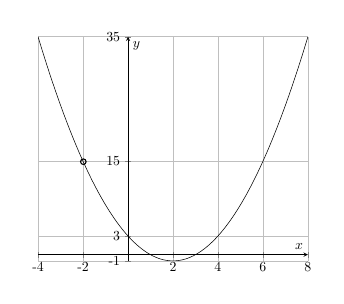
\begin{tikzpicture}[scale=0.5]
\begin{axis}[
    axis lines = middle,
    grid=major,
    legend pos={south west},
    xlabel = {$x$},
    ylabel = {$y$},
    ymin=-1,
    %ymax=250,
    xtick={-4, -2, 2,4,6,8},
    xticklabels={-4,-2, 2,4,6,8},
    ytick={35, 15, -1, 3},
    yticklabels={35, 15, -1, 3}            ]
	\addplot[domain=-4:8, samples=100, color=black] {x*x-4*x+3};
%\addplot[domain=-3.1:2.5, samples=100, color=red] {70*abs(1-2*abs(abs(x)-2))-10*x^2+10*x-70};
	%\addlegendentry{$\text{Рис. 1}$};
\end{axis}
\draw (1.15,2.52) circle (2pt);
\end{tikzpicture}$$
